%%%%%%%%%%%%%%%%% DO NOT CHANGE HERE %%%%%%%%%%%%%%%%%%%% {
\documentclass[12pt,letterpaper]{article} \usepackage{fullpage}
\usepackage[top=2cm, bottom=4.5cm, left=2.5cm, right=2.5cm]{geometry}
\usepackage{amsmath,amsthm,amsfonts,amssymb,amscd}
\usepackage{lastpage}
\usepackage{enumerate}
\usepackage{fancyhdr}
\usepackage{mathrsfs}
\usepackage{xcolor}
\usepackage{graphicx}
\usepackage{listings}
\usepackage{hyperref}

\hypersetup{%
    colorlinks=true,
    linkcolor=blue,
    linkbordercolor={0 0 1}
}

\setlength{\parindent}{0.0in}
\setlength{\parskip}{0.05in}
%%%%%%%%%%%%%%%%%%%%%%%%%%%%%%%%%%%%%%%%%%%%%%%%%%%%%%%%%% }

%%%%%%%%%%%%%%%%%%%%%%%% CHANGE HERE %%%%%%%%%%%%%%%%%%%% {
\newcommand\course{Ilya Sherstyuk}
\newcommand\semester{Spring 2021}
\newcommand\hwnumber{1}                 % <-- ASSIGNMENT #
%%%%%%%%%%%%%%%%%%%%%%%%%%%%%%%%%%%%%%%%%%%%%%%%%%%%%%%%%% }

%%%%%%%%%%%%%%%%% DO NOT CHANGE HERE %%%%%%%%%%%%%%%%%%%% {
\pagestyle{fancyplain}
\headheight 35pt
\lhead{\NetIDa}
\lhead{\NetIDa\\\NetIDb}
\chead{\textbf{\Large CS 148 Set \hwnumber}}
\rhead{\course \\ \semester}
\lfoot{}
\cfoot{}
\rfoot{\small\thepage}
\headsep 1.5em
%%%%%%%%%%%%%%%%%%%%%%%%%%%%%%%%%%%%%%%%%%%%%%%%%%%%%%%%%% }

\begin{document}

% \begin{flushright}Collaborator: Elise Liu\end{flushright}

\textbf{1. Algorithms description}

I closely followed the convolutional perceptron described in class in Lecture 2.
The main idea was to have a set of template traffic light images which are slid over
the image in an attempt to obtain a high dot product which means that the overlapping
part of the image is similar to the template traffic light.

That is meat of the algorithm. In addition, I also normalize the images to have zero
mean and constant standard deviation. Each color channel is normalized independently.
The templates are also normalized, but with respect to the image they came from (for
an example of why this matters, the color ``red'' only has meaning when it is compared
to the blue sky, the green trees, etc).

An alternative was to normalize each image in according to the mean and standard
deviation of the entire data set. I decided it was better to normalize each image
separately, so that something like a image with a slight hue or brightness difference
can still be ``fixed''.

For each template, I also made copies of it in several sizes. This is to deal with the
fact that traffic lights might be closer or further in the test image than it is in
the template image.

A final detail has to do with overlapping detections. When I detect that a new bounding
box has an old bounding box inside it (more precisely, if the center of the old bounding
box is inside the new bounding box), then I remove the old bounding box and extend the
new bounding box to fully encapsulate the old one (this ``merges'' the two boxes).

I didn't try any other algorithms which differ significantly from this one. I mostly
played around with adjusting the dot product threshold, and also selecting good
template images. There was one template image which I thought would be good, but ended
up causing blank regions of the sky to be detected as traffic lights.\\


\textbf{2. Evaluating Performance}

I wrote a short piece of code to visualize the bounding boxes on top of the image,
and I only really manually evaluated the quality of the detections. For the most part,
after making a change to the algorithm, I would run it on the first ten or so pictures
in the dataset and I noted whether there was an improvement or not.

Of course, this is not the greatest way of evaluating performance, as I am essentially
fine-tuning the algorithm on just the first ten images. So it might work OK for those
images but not even the rest of the dataset.
Not to mention that many of the first ten images are in the same setting with only
slight differences, so the actual amount of data which was being effectively ``trained on"
was even less. I also tested the detections in other parts
of the dataset once I felt more or less satisfied with the algorithm, but it would have
been much better to do so at earlier stages too.

As I already said, it would have been better to shuffle or randomly select which images
I was visually evaluating the detections on as I was developing the algorithm. One of
the main reasons I didn't do that is because if there was a ``mistake'' detection,
then I often wanted to check whether the new version of the algorithm fixed that mistake.
Constantly shuffling the images would make these kind of checks harder.\\


\textbf{3. Which Algorithm Performed the Best?}

I've already described the algorithm in the previous question, but I'll use this space
to describe what parameters and templates seemed to work. For my templates, I used
two square photos of the red traffic light. The first template was fairly dim, so the
``light'' part was red and the surrounding part was black, as you might expect.
The second template was much brighter, so the ``light'' part was essentially white,
and the surrounding region had a red glow. This is a bit surprising, but if you look
at the photos you'll see that many of the traffics have white circles surrounded by
red glows.

For the threshold, I found that a good value was $2.5 N$, where $N$ is the number of
pixels in the template image.\\


\textbf{4. Good Examples}

\begin{figure}[htp]
    \centering
    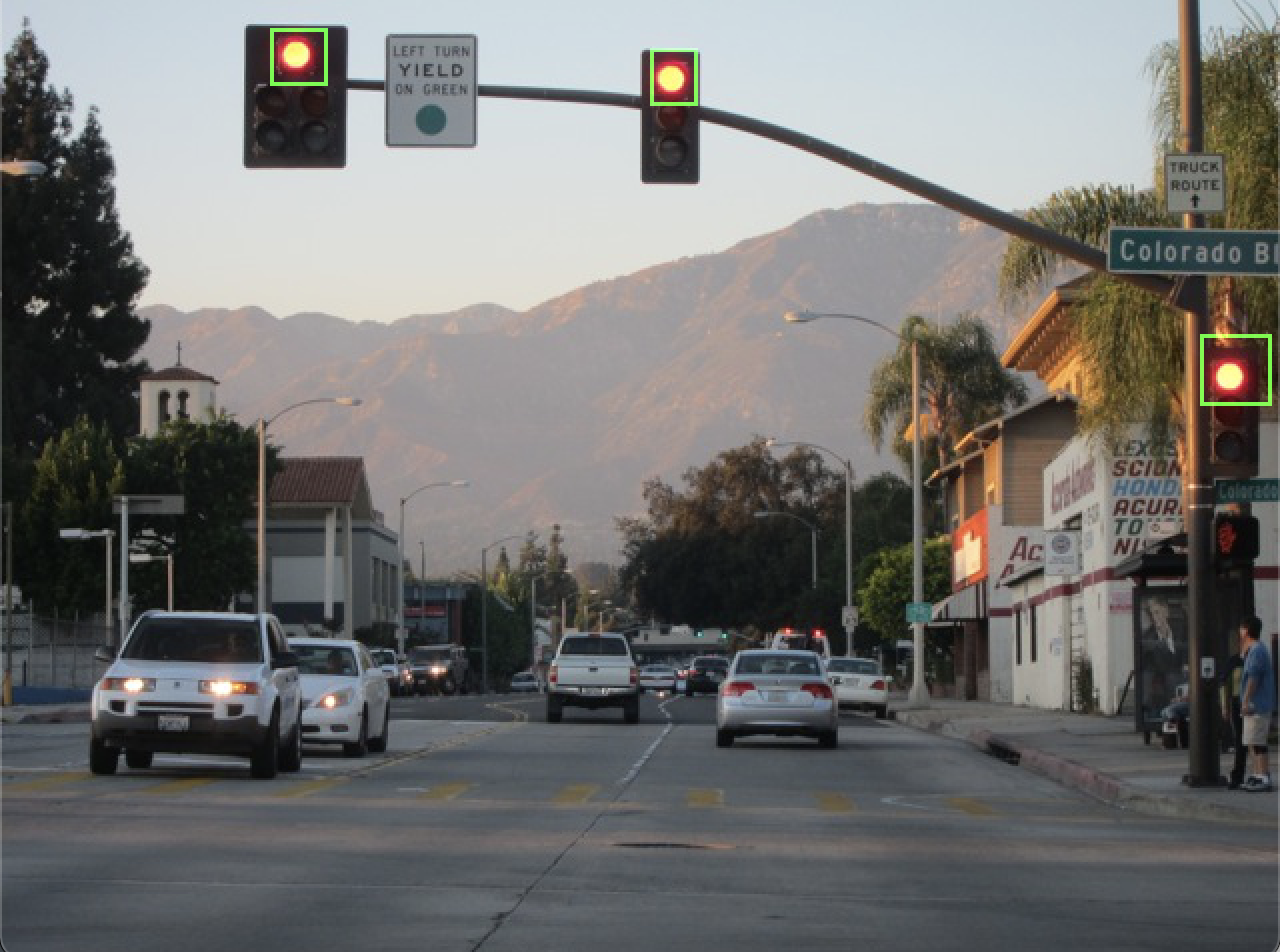
\includegraphics[width=8cm]{img/good1.png}
    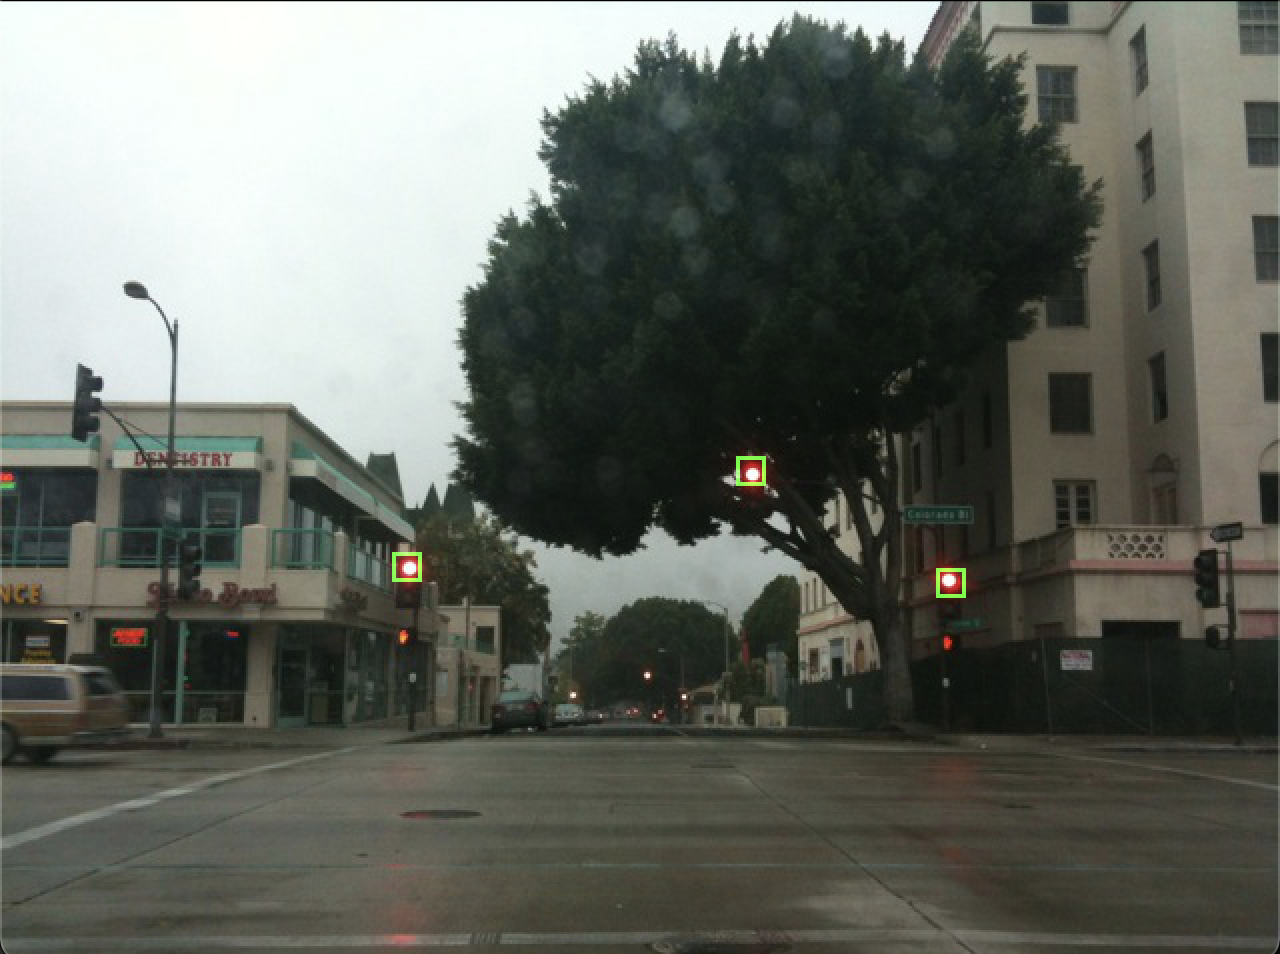
\includegraphics[width=8cm]{img/good2.png}
\end{figure}

Here are two examples where my algorithm succeeded.
The bounding boxes are drawn in green.

I think the left image was easy for the algorithm to get right because the traffic
lights are really close to the camera and have a lot of detail. In most of the other
images, the traffic lights were much smaller, so maybe my templates weren't rescaled
very well to a smaller size, making the smaller lights harder to detect. However, these
lights are nice and large, so there is no trouble detecting them.

In the right image, the traffic lights are pretty nice as well. They aren't as large
but they are still a reasonable size, and they really nicely follow the
``white center, red glow, black shell'' template image. There are some red traffic lights
way in the distance that went undetected, but I wouldn't be too harsh on
my algorithm for not seeing those.\\


\textbf{5. Bad Examples}

\begin{figure}[htp]
    \centering
    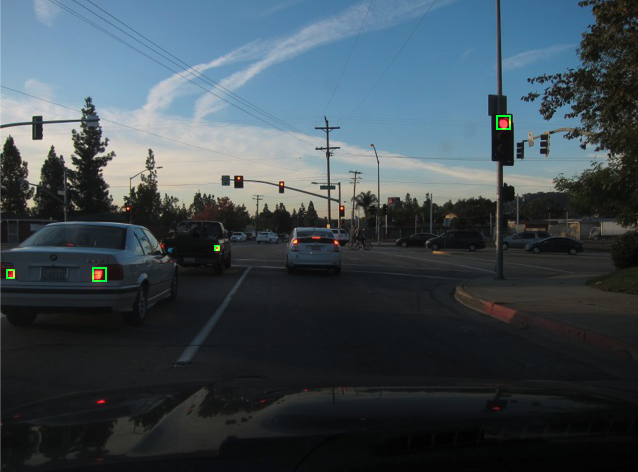
\includegraphics[width=8cm]{img/bad1.png}
    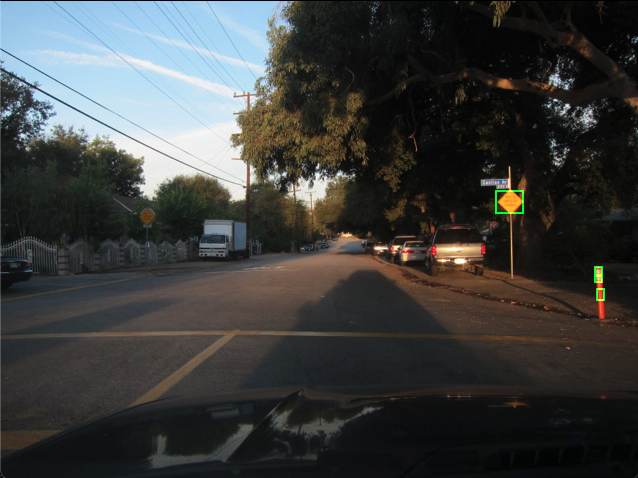
\includegraphics[width=8cm]{img/bad2.png}
\end{figure}

Here are two examples where my algorithm failed.

On the left, we see that the algorithm failed to see some traffic lights, and instead
opted to highlight the cars' tail lights. There are a few reasons this image might be
considered hard. First, the traffic lights are far away, meaning that my template
needed to be shrunk down. The rudimentary resizing function which I wrote might have not
done a good job shrinking the image, so the traffic lights far away slipped away undetected.
The reason that the tail lights are getting detected is because if you only look at
the square which was highlighted, they kind of look like the red traffic signal lights.
Obviously to us they are not, but all the algorithm sees is a bright red round light, not
the surrounding car, so I guess it decided that the tail lights are similar enough to
one of the templates.

On the right, I don't know how it failed so badly. I guess the bright foreground and
dark background of the road sign has a high dot product with one of the templates.
In addition, maybe in the normalization the road sign was made brighter because the
overall image is a bit on the dimmer side.\\

\textbf{6. Possible Improvements}

Currently, the code only works with square templates. This is a large drawback, since
traffic lights are not squares but rectangles, so my square templates only included
the top parts of the traffic lights. This was causing them to often be confused with
tail lights. If the templates had been the entire tall black rectangle of the traffic
light, then the confusion with the tail lights or other red lights in the image would
not have been nearly as likely. The base algorithm of course does not care what shape
the templates are, but in my code I just assumed square templates to make it a bit
easier to implement. But, I think the performance would increase greatly if I were to
add support for non-square templates.\\\\

\textbf{Deliverable \#2}

The code for the best algorithm is in run\_predictions.py and the script
that visualizes the results in this report is called visualize.py.

\end{document}
